\section{RESULTS}
\subsection{Path Deflection in Earth's Magnetic Field}
\label{subsec:31}
We considered a ferromagnetic solid sphere of radius $R=0.5\,\unit{\centi\metre}$ and mass $M=5 \,\unit{\gram}$ carrying an initial magnetic moment $\bm{\mu}(0)=:\bm{\mu}_0$ with direction $\bm{\mu}_0 \| \bm{B}$ and magnitude $\|\bm{\mu}_0\|=:\mu_0=1.0\,\unit{\ampere\metre\squared}$ comparable to a real Neodymium magnet of this size~\cite{Amrani2015}. The solid sphere rolls on an incline with opening angle $\varphi=20^\circ$ in Earth's magnetic field $\bm{B}$. Data on $\bm{B}$ was obtained from the World Magnetic Model~\cite{ncei26}. Simulation time was set to $\Delta t=0.5\,\unit{\second}$ at a discretization of $\delta t=10^{-5} \,\unit{\second}$. The coordinate system is centered at the center of mass at $t=0 \, \unit{s}$ and the incline is rotated such that the $\bm{e}_x$-direction points eastwards, the $\bm{e}_y$-direction points northwards, and the $\bm{e}_z$-direction points up. The influence of the magnetic field was measured by the $x$-coordinate after $0.5 \, \unit{\second}$ because without an external field, the sphere's path would be contained in the $yz$-plane.
\begin{figure}[htbp]
    \centering
    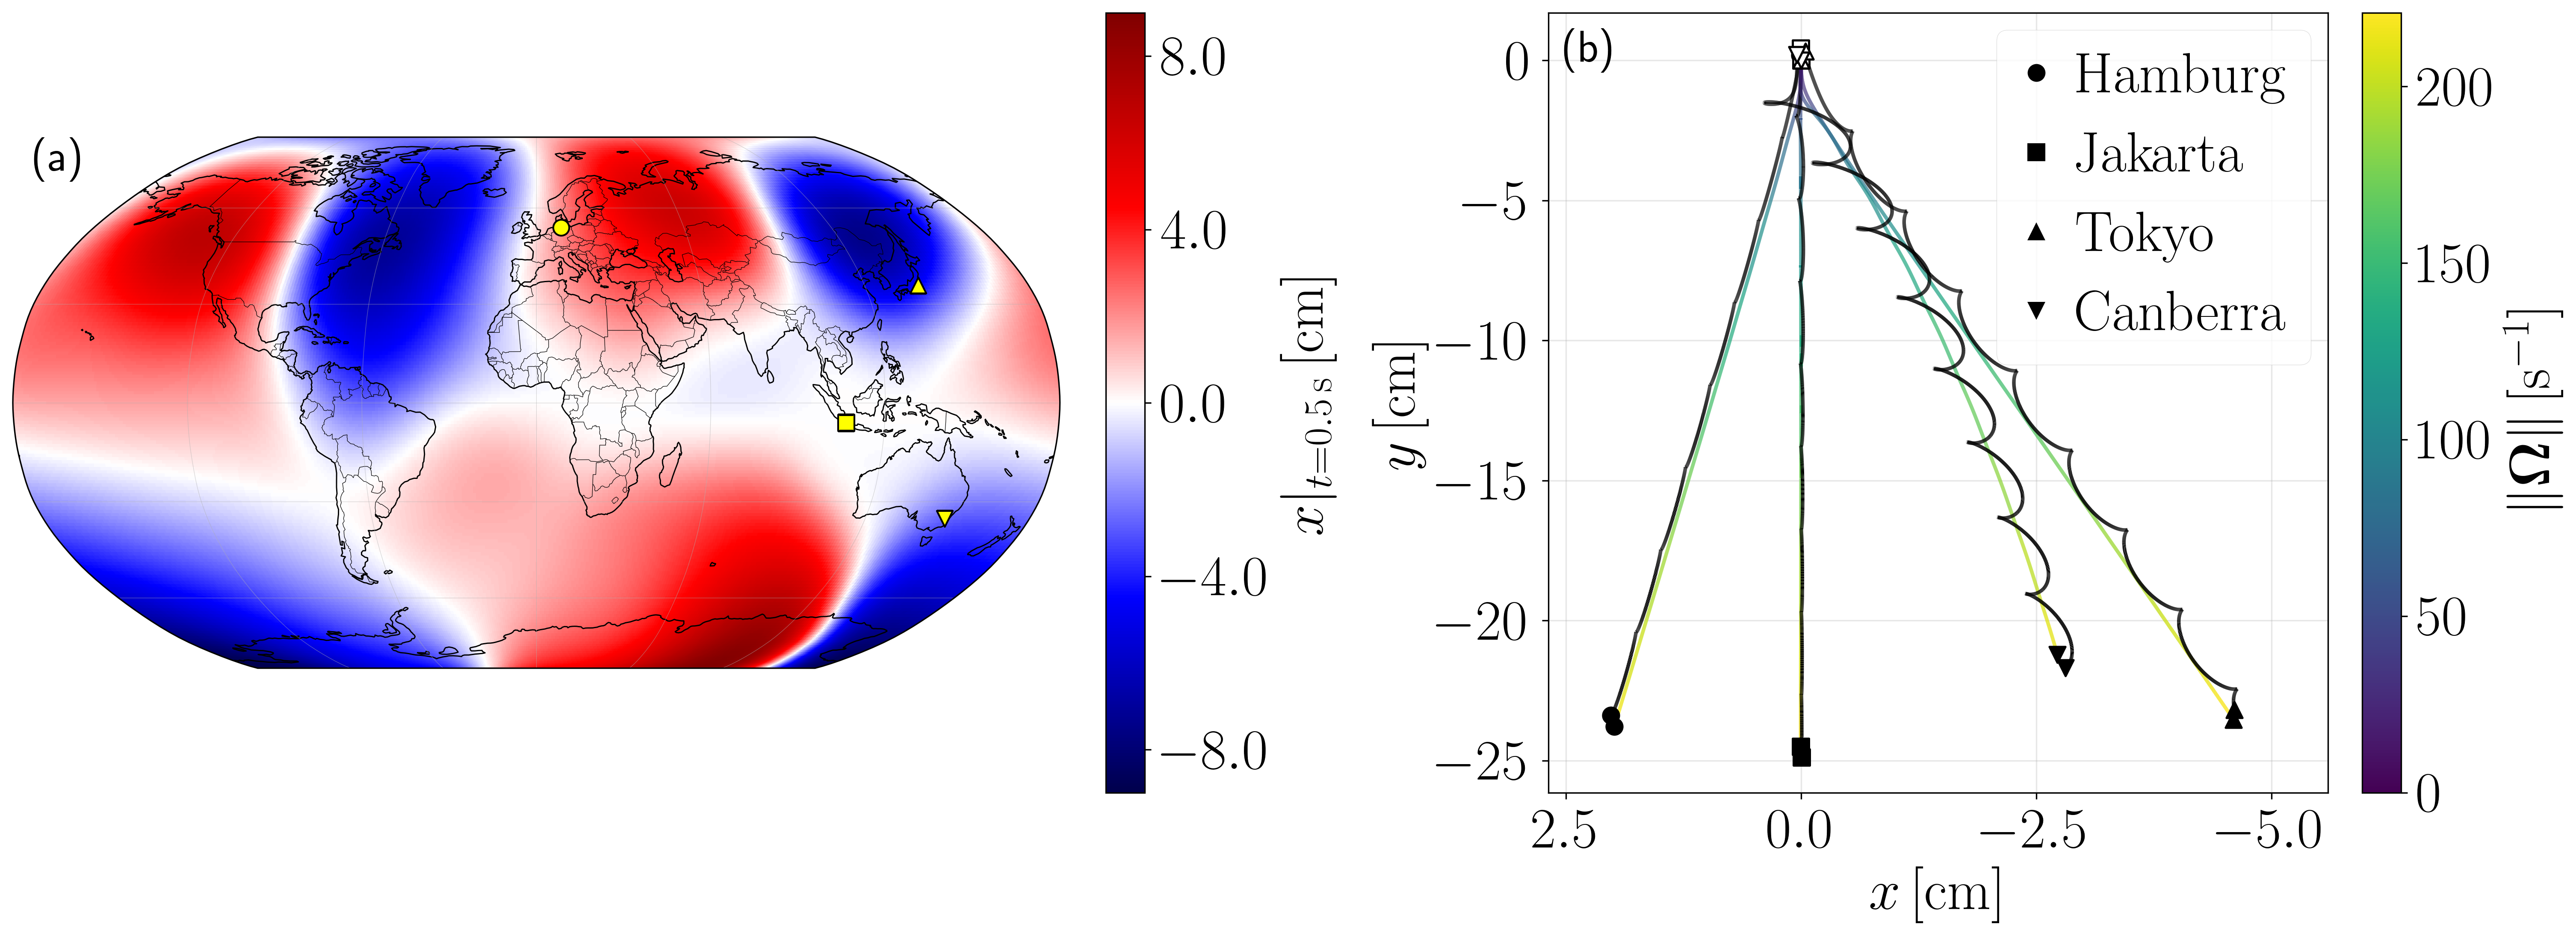
\includegraphics[width=\textwidth]{k.png}
    \caption{Robinson-projection of the deviation in $x$ depending on latitude and longitude (a) and selected trajectories in the $xy$-plane for different places on Earth (b). In (b), smooth lines represent the center-of-mass-trajectory colored by total angular velocity, while the black lines represent the projection of the direction of the magnetic moment vector normed to the sphere's radius. Initially, the magnetic moment $\bm \mu _0$ and the magnetic field $\bm B$ are aligned: $\bm \mu _0 \| \bm{B}$. The four trajectories are animated in Ref.~\cite{SM}.}
    \label{fig:k}
\end{figure} 
As seen in Fig. \ref{fig:k}, we observe a significant deflection of the solid sphere from an ideal straight path as it would be observed without any magnetic interaction. The strong dependence of the trajectories on the direction of the outer magnetic field leads us to predict that in a comparable experiment carried out in a laboratory, the results will vary noticeably with the location of the laboratory. 
\subsection{Influence of Magnetic Moment and External Field}
Aiming to understand the observed dependence of the system on the external field and the magnetic moment, we parametrized
\begin{equation}
    \bm{\mu}_0= \mu_0(\sin \psi \sin \theta, \sin \psi \cos \theta, \cos \psi)^\top
\end{equation}
and 
\begin{equation}
    \bm{B}=B(\sin \overline{\psi} \sin \overline{\theta}, \sin \overline{\psi} \cos \overline{\theta}, \cos \overline{\psi})^\top
\end{equation}
with azimuthal angles $\theta, \overline{\theta}$ and polar angles $\psi, \overline{\psi}$. First, we considered $\psi=\overline{\psi}=\frac{\pi}{2}$ and $\theta, \overline{\theta} \in \left[ -\pi, \pi\right]$, varying $\mu_0 \in [0.0 \,\unit{\ampere\metre\squared}, 2.5 \,\unit{\ampere\metre\squared}]$ while keeping $\bm{B}=c_{\bm{B}} \bm{e}_z$ fixed for $c_{\bm{B}}:=5 \cdot 10^{-5} \, \unit{\tesla}$. To examine the behavior under exchange of $\bm{B}$ and $\bm{\mu}_0$, we also varied $B \in [0.0\,\unit{\tesla}, 2.5 \,\unit{\tesla}]$ while keeping $\bm{\mu}_0=c_{\bm{\mu}_0}\bm{e}_z$ for $c_{\bm{\mu}_0}:=5 \cdot 10^{-5} \, \unit{\ampere\metre\squared}$ constant. The influence of the magnetic torque on the trajectory was again measured by the value of the $x(t)$-coordinate after $\Delta t= 1 \,\unit{\second}$ of simulation time at an inclination opening angle of $\varphi = 10^\circ$. Results are shown in Fig.~\ref{fig:f1} and Fig.~\ref{fig:f2}.
\begin{figure}[htbp]
    \centering
    
\includegraphics[width=\textwidth]{f1.pdf}
    \caption{Final deviation $x|_{t=1\,\unit{s}}$ in relation to azimuthal angles $\theta, \overline{\theta}$ for different $\mu_0$ in (a) and different $B$ in (b). All graphs are point symmetric with respect to the origin. Critical points can be observed in both (a) and (b). Moreover, the critical points shift towards the origin and the maximal deviation increases with modulus in (a). The latter can also be seen in (b), yet the extrema do not follow a clear pattern for increasing $B$ like they do in (a).}
    \label{fig:f1}
\end{figure}
Fig.~\ref{fig:f1} shows the final $x$-deviation of the solid sphere from the straight trajectory as a function of the initial orientation of the magnetic moment and the magnetic field. It can be seen in (a) that,  when varying $\bm{\mu}_0$, two critical points, i.e., points at which the first derivative vanishes, appear in all deviation curves. For very low values of $\mu$, the absolute deviation decreases smoothly after the critical points are reached. For higher values of $\mu$, the behavior after the critical points becomes erratic. Conversely, varying $B$ does not cause erratic behavior to appear, as seen in Fig.~\ref{fig:f1}~(b). The absolute deviation generally increases with increasing $B$, but multiple pairs of critical points emerge. This behavior can be understood by looking at the selected trajectories in Fig.~\ref{fig:f2}.
\begin{figure}[htbp]
    \centering
    
\includegraphics[width=\textwidth]{f2.pdf}
    \caption{Trajectories on the $xy$-plane for selected moduli of $\bm{\mu}_0$ in (a,b) and $\bm{B}$ in (c,d). In (a) and (b), the curvature of trajectories increases with $\mu_0$ and $\theta$, yet the total deviation decreases for high values of $\theta$. In contrast, the paths in (b) start to loop around the origin for high values of $|\theta|$. In (c) and (d), the trajectories are strongly curved towards $x=0$, crossing over for high values of $|\overline{\theta}|$. Animations of exemplary trajectories are provided in Ref.~\cite{SM}.}
    \label{fig:f2}
\end{figure}
Comparing Fig.~\ref{fig:f1}~(a) with Fig. \ref{fig:f2}~(a), we see that the curvature for low values of $\mu$ increases with $|\theta|$. However for $|\theta|>\frac{\pi}{2}$, the downward rolling is at first opposed by the magnetic torque reducing the total distance rolled and hence also the total deviation. Fig.~\ref{fig:f2}~(b) reveals that this is caused by the magnetic torque overcompensating the gravitational torque, causing the sphere to loop around the origin. Fig.~\ref{fig:f2} (c,d) shows that the solid sphere twists around the $x=0$ line. Depending on the azimuthal angle $\overline{\theta}$, the solid sphere crosses the line. This divides the graphs in Fig.~\ref{fig:f1}~(b) into two regions: For values of $\overline{\theta}$ between around $\frac{-\pi}{4} \, \unit{rad}$ and $\frac{\pi}{4} \, \unit{rad}$, the sphere is increasingly deflected from the straight path with increasing $|\overline{\theta}|$. At the first pair of critical points $\overline{\theta} \approx \pm \frac{\pi}{4} $, the trajectories start to curve towards the $x=0$-line again. The pair of zeros at $\overline{\theta}=\pm \frac{\pi}{2} \, \unit{rad}$ represents the point at which the path ends exactly on that line. For $|\overline{\theta}| > \frac{\pi}{2}$, the sphere crosses over $x=0$, causing the deviation curves to invert. In general, the twisting motion seen in Fig.~\ref{fig:f2}~(c,d) also becomes tighter around the $x=0$ line with increasing values of $|\overline{\theta}|$. This explains the decrease of total deviation observed for high values of $B$ in Fig.~\ref{fig:f1}~(b).\\
In Fig.~\ref{fig:g} we set $B=5 \cdot 10^{-5}\,\unit{\tesla}$, $\mu_0 = 1.0\,\unit{\ampere\metre\squared}$, $\theta=\overline{\theta}=0^\circ$, and $\overline{\psi}=0^\circ$, varying $\psi \in [-\pi,\pi)$. In addition, we repeated the simulations with the roles of $\bm{\mu}$ and $\bm{B}$ exchanged, also seen in Fig.~\ref{fig:g}. All other simulation parameters were kept from the previous simulation. Since this causes no deviation in $x(t)$, we used the value of the $y(t)$-coordinate after $\Delta t = 1\,\unit{\second}$ as measure for the influence of the magnetic torque.
\begin{figure}[htbp]
    \centering
    
\includegraphics[width=\textwidth]{g.pdf}
    \caption{Final coordinate of the sphere $y|_{t=1\,\unit{s}}$ in relation to polar angles $\psi, \overline{\psi}$ in (a) and $y(t)$-curves for representative values of $\psi$ in (b). The grey dotted curve in (a) corresponds to exchanged roles of $\mu_0$ and $B$. In (a), three different regions are discernible: a high-deviation, a low-deviation, and an intermediate region. For each, a representative $y$-trajectory is shown in (b).  Exchanging $\bm{\mu}$ and $\bm{B}$ only causes a reflection of the curve in (a) around $\psi=0$. Videos of the three representative trajectories are contained in Ref.~\cite{SM}.}
    \label{fig:g}
\end{figure}
Fig.~\ref{fig:g} clearly shows that for polar angles between about $\frac{-3\pi}{4}\,\unit{rad}$ and $0\,\unit{rad}$, the magnetic force fully dominates over the gravitational force, thus the solid sphere oscillates in the $yz$-plane without rolling down as seen in (b). This behaviour transitions to oscillations which are eventually overcome by gravity at a specific point in time. The more favourable the downhill motion is for the total magnetic energy, the sooner this critical point is reached. In contrast to Fig.~\ref{fig:f1}, the mirror symmetry under exchange of $\bm{\mu}$ and $\bm{B}$ is readily explained by the fact that we can write $\bm{\mu}(t)=\mu(0, \sin \psi(t), \cos \psi(t))^\top$ since $\bm{\mu}(t)$ remains always in the $yz$-plane. The magnetic torque thus reduces to
\begin{equation}
    \bm{\tau}_\text{em}(t)=\mu B\sin \psi(t) \bm{e}_x.
\end{equation}
Exchanging the roles of $\bm{B}$ and $\bm{\mu}$ simply means to reverse the angle $\psi(t)$ to $2 \pi - \psi(t)$, causing the observed sign flip of $\bm{\tau}_\text{em}$ as sinus is an odd function. The immediate difference to the conditions in Fig.~\ref{fig:f1} is that no torque breaking the mirror symmetry of the system with respect to the $yz$-plane can occur. This constrains $\bm{\mu}$ to the $yz$-plane, reducing the effective rotational degrees of freedom to one, parametrized by an antisymmetric function.
